%!TEX root = /Users/Nikolaj/Developer/GPU-Project/Report/Report.tex

Now that it has been established that the solution produces satisfactory results it is time to examine the increase in speed that the solution provides. Four different performance tests were performed each one providing a different insight into how this solution was improved compared to original C\# implementation. The graphs depicted in this section are all from the Gpulab06 machine because the performance of this machine was the best. Full performance tests for all machines can be found in Appendix \ref{app:graphs}. Note that the number of steps taken per year in the middle model is 2 for all test.\\

\subsection{Variable $x$}

Each step in the outer model takes equally long time to complete. This is because the number of steps taken in the middle and the inner model is constant as long as $h$ is constant. 
The relationship between the number of steps to take in the outer model and the time it takes to solve it can therefore be expressed as a linear equation. 
The number of steps in the outer model is solved from $120-x$ to 0 the $x$-value is proportional with the number of steps. This means that the running time is also a linear equation proportional with $x$.

It is important to show that our solution is fast no matter what values are chosen. Changing $g$ and $r$ will have no performance effect and is therefore not included in the tests.

\begin{figure}[ht!]
\begin{center}
	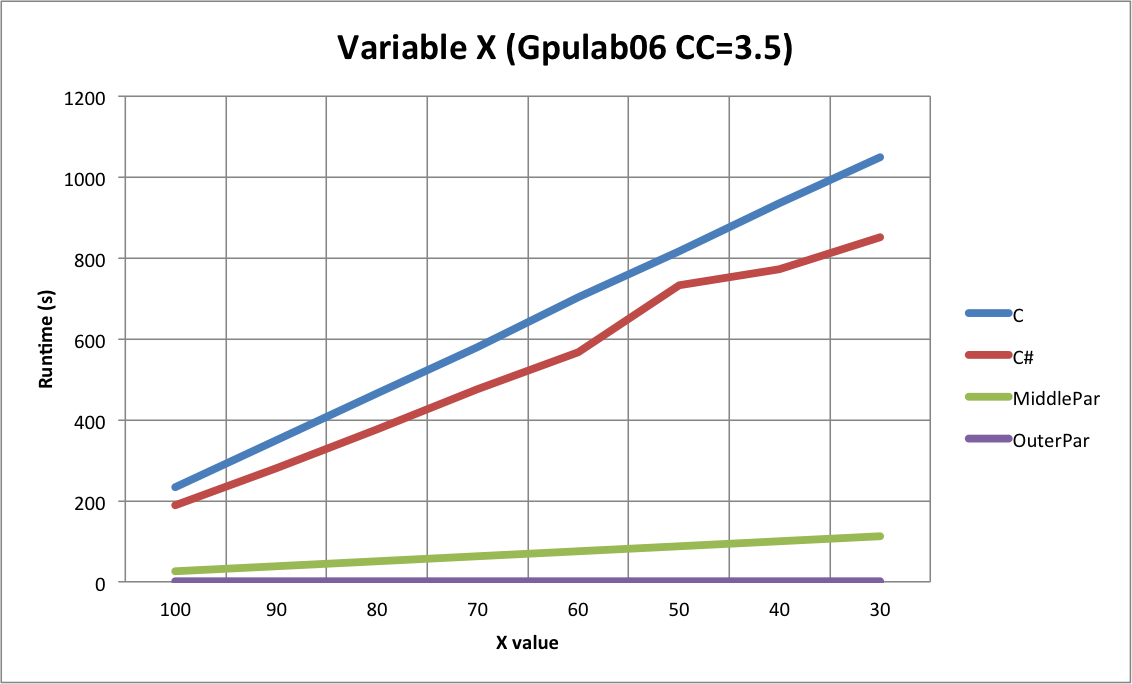
\includegraphics[width=\textwidth]{img/Gpulab-varx35.png}
\end{center}
\caption{The impact of changing the $x$ value on the Gpulab06 machine}
\label{variablex}
\end{figure}

When the $x$ value rises the runtime naturally increases because the outer model is solved from $120-x$ to 0. The lower the $x$ value the more steps needed. Our OuterPar solution is faster than the other implementations, and even though the runtime also increases for this solution it does not increase significantly. The results showed up to 665 times faster runtime compared to the original C\# solution.

\subsection{Variable Stepsize}
One of the advantages of using a 4th order Runge-Kutta solver is that an appropiate number of steps per year can be chosen to adjust the precision at the cost of an increase in running time. While increasing the steps per year will increase the running time in our implementation the increase is quite small compared to the C and C\# implementations.

\begin{figure}[ht!]
\begin{center}
	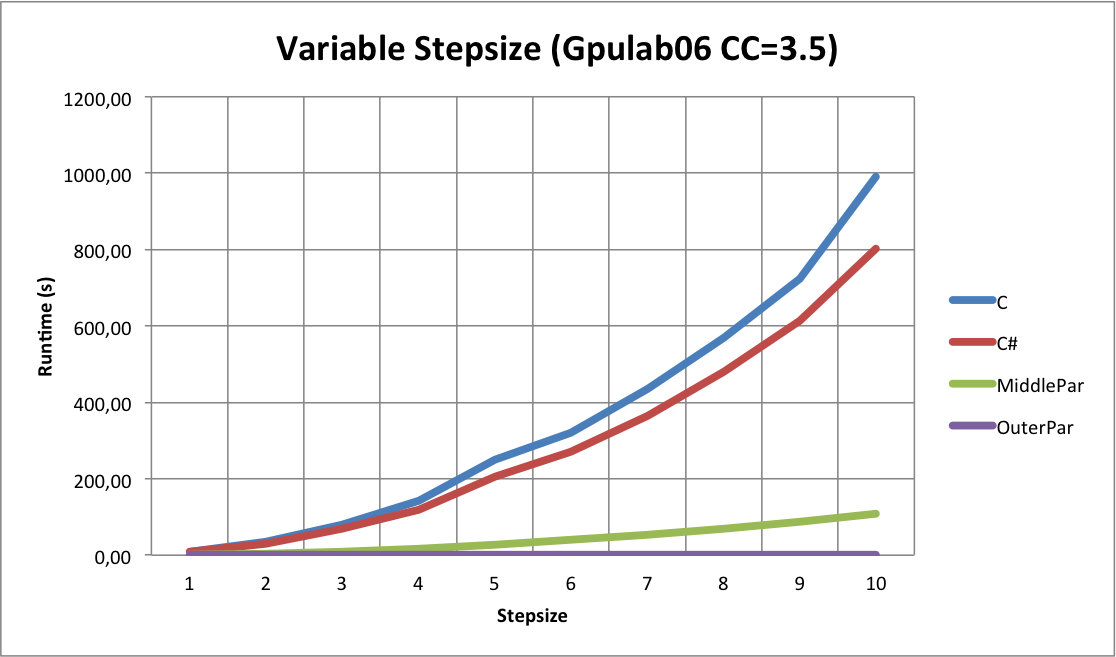
\includegraphics[width=\textwidth]{img/Gpulab-stepsize35.png}
\end{center}
\caption{The impact of changing the stepsize on the Gpulab06 machine}
\label{variablestepsize}
\end{figure}

Increasing the number of steps per year does increase the running time as expected but our OuterPar solution is superior in every test we performed on all the machines. The results showed up to 680 times faster running times compared to the original C\# implementation.

\subsection{Variable Threads per Block}
Since the number of threads per block is set at compile time in the CUDA implementations it is interesting to test what impact different amounts have on the performance.

\begin{figure}[ht!]
\begin{center}
	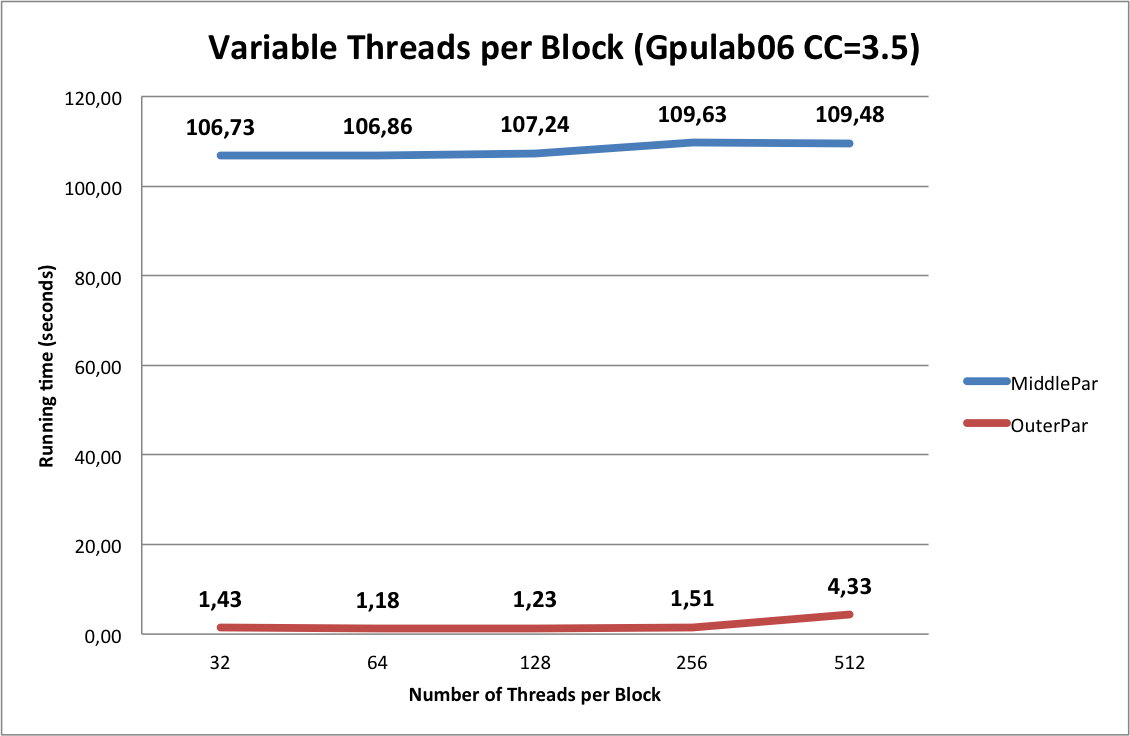
\includegraphics[width=\textwidth]{img/Gpulab-tpb35.png}
\end{center}
\caption{The impact of changing the threads per block on the Gpulab06 machine}
\label{ThreadsPerBlockGraph}
\end{figure}

\noindent As seen in Fig. \ref{ThreadsPerBlockGraph}, the slowest configuration is 512 threads per block. This is expected since the Gpulab06 GPU has a hardware limit of 2048 threads per SMP meaning that it schedules (2048 / 512) = 4 blocks at a time even though the hardware can schedule as many as 16. To increase performance, the amount of threads per block has to be lowered to yield more blocks and thus a better utilization of the SMPs. This fact explains the drastic improvement from 512 to 256 and from 256 til 128, at which the number of blocks reaches the exact hardware limit. Lowering the count further to 64 threads per block, however, seems to keep improving performance even though we already reached 16 blocks. \\

In this case, the explanation should be sought in the way SMPs divide threads of the executing blocks into warps. With a configuration of 64 threads per block, the SMP splits each block into 2 warps of 32 threads each instead of 4, 8 or 16 warps with 128, 256 and 512 threads per block respectively. The lower amount of warps that each block is split into, the fewer warps will have to leave the SMP when a single thread from a block is taking a long time to execute and cause the entire block to leave the SMP. This results in a faster exchange of blocks which means that the amount of threads in an SMP that is actually doing some work increases. \\

Using this line of thought, one could argue that having just 32 threads per block should be even faster. Considering the work that each thread is doing this is not the case. The middle model is solved from 119 to 1 yielding 238 steps in total with 2 steps per year. Since each step is taken care of by a thread, allocating more than 238 threads leaves som threads with no work to do while fewer than 238 require each thread to take more than one step. Looking at the graph, it is clear that the best balance between workload and number of threads lies somewhere between 32 and 64 threads per block on the Gpulab06 machine.

\subsection{Register Spilling}
It is worth mentioning that each kernel thread uses 68 registers which is more than the available limit on Nvidia GPUs with compute capability 3.0 or lower. Therefore, to reproduce these results, one should avoid register spilling by including -arg=sm\_35 when compiling the code with nvcc. In this way, the compiler will know that the code is going to run on GPUs with 255 registers available per thread. \\

The program will stop functioning if it is compiled with a compute capability between 2.0 and 3.0 and run with more than 512 threads per block because of the register limit. If it is run with less than 512 threads per block it will function but the runtime will be significantly reduced because of register spilling.

\subsection{Exp vs Pow}
After running all performance tests we discovered that the use of \texttt{exp} instead of \texttt{pow} in both the C and C\# implementation improved the running time substantially. Apparantly the \texttt{exp} function is much faster for calculation, and a few short tests showed an improvement i execution time between 20\% and 50\%. A future improvement should use \texttt{exp} instead of \texttt{pow}, as the change had no impact on the final reserve estimated by C and C\#.

\subsection{Results}
Looking at Fig. \ref{variablex} and Fig. \ref{variablestepsize} it is clear that they are not all perfectly linear even though it is mandated by the theory. The reason for this inconsistency is most likely that the implementations are run a computer whose resources are not allocated entirely for the program meaning that the amount of resources available for the program could vary during the execution. \\

From this section, we can conclude that both of the parallelized CUDA implementations are superior in running time compared to the C and C\# implementations. Furthermore, the running time of the OuterPar implementation surpassed the running time of the MiddlePar implementation in all tests performed.